\section{The perception-distortion tradeoff}\label{sec:tradeOff}
We saw that for any distortion measure, a low distortion does not generally imply good perceptual-quality. An interesting question, then, is: What is the best perceptual quality that can be attained by an estimator with a prescribed distortion level?
\begin{definition}
The perception-distortion function of a signal restoration task is given by
\begin{equation}\label{eq:fAlpha}
P(D) = \min_{p_{\hat{X} \vert Y}} \, d(p_X,p_{\hat{X}}) \quad \text{s.t.} \quad  \E[\Delta(X,\hat{X})] \le D,
\end{equation}
where $\Delta(\cdot,\cdot)$ is a distortion measure and $d(\cdot,\cdot)$ is a divergence between distributions.
\end{definition}
In words, $P(D)$ is the minimal deviation between the distributions $p_X$ and $p_{\hat{X}}$ that can be attained by an estimator with distortion $D$.
To gain intuition into the typical behavior of this function, consider the following example.
\begin{example}\label{ex:scalarGaussian}
Suppose that $Y=X+N$, where $X \sim \mathcal{N}(0,1)$ and $N \sim \mathcal{N}(0,\sigma_N^2)$ are independent. Take $\Delta(\cdot,\cdot)$ to be the square-error distortion and $d(\cdot,\cdot)$ to be the KL divergence. For simplicity, let us focus on estimators of the form $\hat{X}=aY$. In this case, we can derive a closed form solution to Eq.~\eqref{eq:fAlpha} (see Appendix \ref{ap:scalarGaussian}), which is plotted for several noise levels $\sigma_N$ in Fig.~\ref{fig:scalarGaussianExample}. As can be seen, the minimal attainable $d_{\text{KL}}(p_X,p_{\hat{X}})$ drops as the maximal allowable distortion (MSE) increases. Furthermore, the tradeoff is convex and becomes more severe at higher noise levels $\sigma_N$.
\end{example}

\begin{figure}
	\begin{center}
        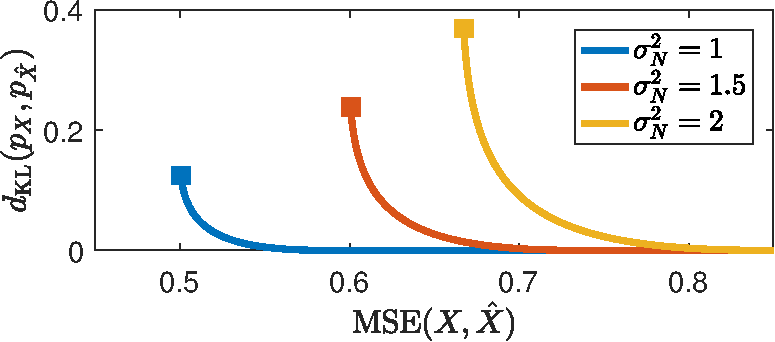
\includegraphics[width=0.9\linewidth]{figures/scalarGaussian.pdf}
	\end{center}
	\caption{\textbf{Plot of Eq.~\eqref{eq:fAlpha} for the setting of Example~\ref{ex:scalarGaussian}}. The minimal attainable KL distance between $p_X$ and $p_{\hat{X}}$ subject to a constraint on the maximal allowable MSE between $X$ and $\hat{X}$. Here, $Y=X+N$, where $X \sim \mathcal{N}(0,1)$ and $N \sim \mathcal{N}(0,\sigma_N)$, and the estimator is linear, $\hat{X}=aY$. Notice the clear trade-off: The perceptual index ($d_{\text{KL}}$) drops as the allowable distortion (MSE) increases. The graphs cut-off at the MMSE (marked by a square).}
	\label{fig:scalarGaussianExample}
\end{figure}

In general settings, it is impossible to solve~\eqref{eq:fAlpha} analytically. However, it turns out that the behavior seen in Fig.~\ref{fig:scalarGaussianExample} is typical, as we show next (see proof in Appendix \ref{ap:convexityProof}).


\begin{theorem}[The perception-distortion tradeoff]\label{lem:convexity}
Assume the problem setting of Section~\ref{sec:perceptionDistortion}. If $d(p,q)$ of \eqref{eq:PerceptualQualityIndex} is convex in its second argument\footnote{That is, $d(p,\lambda q_1 + (1-\lambda) q_2) \le \lambda d(p,q_1) + (1-\lambda) d(p,q_2)$ for any three distributions $p,q_1,q_2$ and any $\lambda \in [0,1]$.},
then the perception-distortion function $P(D)$ of \eqref{eq:fAlpha} is
\vspace{-0.15cm}
\begin{enumerate}
	\item monotonically non-increasing;
	\item convex.
\end{enumerate}
\end{theorem}

Note that Theorem~\ref{lem:convexity} requires no assumptions on the distortion measure $\Delta(\cdot,\cdot)$. This implies that a tradeoff between perceptual quality and distortion exists for \emph{any distortion measure}, including \eg MSE, SSIM, square error between VGG features \cite{johnson2016perceptual,ledig2016photo}, etc. Yet, this does not imply that all distortion measures have the same perception-distortion function. Indeed, as we demonstrate in Sec.~\ref{sec:practicalMethod}, the tradeoff tends to be less severe for distortion measures that capture semantic similarities between images.

The convexity of $P(D)$ implies that the tradeoff is more severe at the low-distortion and at the high-perceptual-quality extremes. This is particularly important when considering the TV divergence which is associated with the ability to distinguish between real vs.~fake images (see Sec.~\ref{sec:RelatedWorkPerceptualQuality}). Since $P(D)$ is steeper at the low-distortion regime, any \emph{small} improvement in distortion for an algorithm whose distortion is already low, must be accompanied by a \emph{large} degradation in the ability to fool a discriminator. Similarly, any \emph{small} improvement in the perceptual quality of an algorithm whose perceptual index is already low, must be accompanied by a \emph{large} increase in distortion. Let us comment that the assumption that $d(p,q)$ is convex, is not very limiting. For instance, any $f$-divergence (\eg KL, TV, Hellinger, $\mathcal{X}^2$) as well as the Renyi divergence, satisfy this assumption \cite{csiszar2004information,van2014renyi}. In any case, the function $P(D)$ is monotonically non-increasing even without this assumption.

\subsection{Bounding the Perception-Distortion function}\label{sec:bounding}

Several past works attempted to answer the question: What is the minimal attainable distortion $D_{\min}$ in various restoration tasks? \cite{levin2011natural,levin2012patch,chatterjee2010denoising,chatterjee2011practical,baker2002limits}. This corresponds to the value 
\begin{equation}\label{eq:Dmin}
D_{\min} =  \min_{p_{\hat{X}|Y}} \E[\Delta(X,\hat{X})],
\end{equation}
which is the horizontal coordinate of the leftmost point on the perception-distortion function. However, as the minimum distortion estimator is generally not distribution preserving (Sec.~\ref{sec:arbitrary_dist}), an important complementary question is: What is the minimal distortion that can be attained by an estimator \emph{having perfect perceptual quality}? This corresponds to the value
\begin{equation}\label{eq:Dmax}
D_{\max} =  \min_{p_{\hat{X}|Y}} \E[\Delta(X,\hat{X})] \quad \text{s.t.} \quad p_{\hat{X}} = p_X,
\end{equation}
which is the horizontal coordinate of the point where the perception-distortion function first touches the horizontal axis (see Fig.~\ref{fig:minMaxDist}).

Observe that perfect perceptual quality ($p_{\hat{X}} = p_X$) is always attainable, for example by drawing $\hat{x}$ from $p_X$ independently of the input $y$. 
This method, however, ignores the input and is thus not good in terms of distortion. 
It turns out that perfect perceptual quality can generally be achieved with a significantly lower MSE distortion, as we show next  (see proof in Appendix \ref{ap:boundProof}).

\begin{figure}
	\begin{center}
		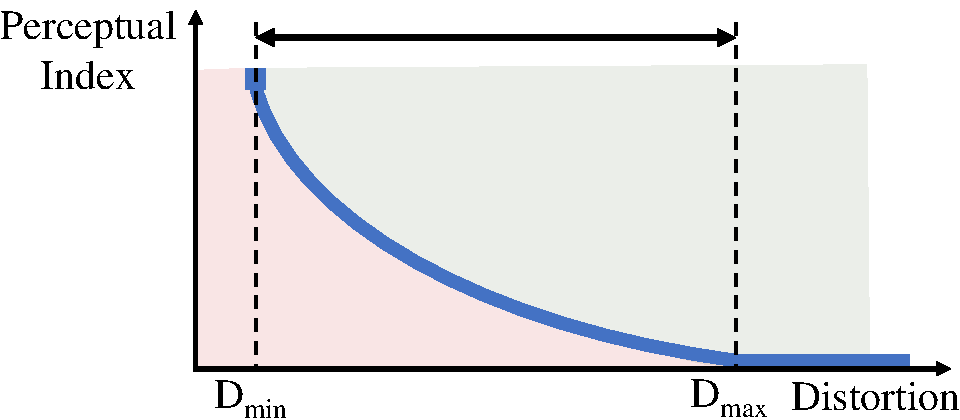
\includegraphics[width=0.85\linewidth]{figures/minMaxDist.pdf}
	\end{center}
	\caption{\textbf{Bounding the perception-distortion function.} The distance between $D_{\min}$ and $D_{\max}$ is the increase in distortion which is needed to obtain perfect perceptual quality. For the MSE, Theorem \ref{thm:bound} proves this will never be more than a factor of $2$ (which is $3$dB in terms of PSNR).}
	\label{fig:minMaxDist}
\end{figure}

\begin{theorem}\label{thm:bound}
	For the square error distortion $\Delta(x,\hat{x}) = \|\hat{x}-x\|^2$,
	\begin{equation}
	D_{\max}\leq 2D_{\min},
	\end{equation}	
	where $D_{\min}$ and $D_{\max}$ are defined by \eqref{eq:Dmin} and \eqref{eq:Dmax}, respectively. This bound is attained by the estimator $\hat{X}$ defined through
\begin{equation}\label{eq:xpost}
p_{\hat{X}|Y}(x|y) = p_{X|Y}(x|y),
\end{equation}
which achieves $p_{\hat{X}}=p_X$ and has an MSE of $2D_{\min}$.
\end{theorem}

In simple words, Theorem \ref{thm:bound} states that one would never need to sacrifice more than $3$dB in PSNR to obtain perfect perceptual quality. This can be achieved by drawing $\hat{x}$ from the posterior distribution $p_{X|Y}$. Interestingly, such a degradation was indeed incurred by all super-resolution methods that achieved state-of-the-art perceptual quality to date. This can be seen in Fig.~\ref{fig:noRefMethods1}, where the RMSE of the algorithms with the lowest perceptual index is nearly a factor of $\sqrt{2}$ larger than the RMSE of the methods with the lowest RMSE (see also \cite{ledig2016photo,sajjadi2017enhancenet}). However, note that this bound is generally not tight. For example, in the scalar Gaussian toy example of Fig.~\ref{fig:scalarGaussianExample}, $D_{\max}$ can be quite smaller than $2D_{\min}$, depending on the noise level.

\subsection{Connection to rate-distortion theory}\label{sec:rateDistortion}
The perception-distortion tradeoff is closely related to the well-established rate-distortion theory \cite{cover2012elements}. This theory characterizes the tradeoff between the bit-rate required to communicate a signal, and the distortion incurred in the signal's reconstruction at the receiver. More formally, the rate-distortion function of a signal $X$ is defined by
\begin{equation}\label{eq:rateDistortion}
R(D) = \min_{p_{\hat{X} \vert X}} \, I(X;\hat{X}) \quad \text{s.t.} \quad  \E[\Delta(X,\hat{X})] \le D,
\end{equation}
where $I(\!X;\hat{X}\!)$ is the mutual information between $X$ and $\hat{X}$.

There are, however, several key differences between the two tradeoffs. First, in rate-distortion the optimization is over all conditional distributions $p_{\hat{X} \vert X}$, \ie given the \emph{original} signal. In the perception-distortion case, the estimator has access only to the degraded signal $Y$, so that the optimization is over the conditional distributions $p_{\hat{X} \vert Y}$, which is more restrictive. In other words, the perception-distortion tradeoff depends on the degradation $p_{Y|X}$, and not only on the signal's distribution $p_X$ (see Example~\ref{ex:scalarGaussian}). Second, in rate-distortion the rate is quantified by the mutual information $I(X;\hat{X})$, which depends on the joint distribution $p_{X,\hat{X}}$. In our case, perception is quantified by the similarity between $p_X$ and $p_{\hat{X}}$, which does not depend on their joint distribution. Lastly, mutual information is inherently convex, while the convexity of the perception-distortion curve is guaranteed only when $d(\cdot,\cdot)$ is convex.

While the two tradeoffs are different, it is important to note that perceptual quality does play a role in lossy compression, as evident from the success of recent GAN based compression schemes \cite{tschannen2018deep, agustsson2018generative, santurkar2018generative}. Theoretically, its effect can be studied through the rate-distortion-perception function \cite{blau2019rethinking,matsumoto2018introducing,matsumoto2018rate}, which is an extension of the rate-distortion function \eqref{eq:rateDistortion} and the perception-distortion function \eqref{eq:fAlpha}, characterizing the triple tradeoff between rate, distortion, and perceptual quality. 

\section{Traversing the tradeoff with a GAN}\label{sec:WGAN}
There exists a systematic way to design estimators that approach the perception-distortion curve: Using GANs. Specifically, motivated by \cite{ledig2016photo,pathak2016context,yeh2017semantic,sajjadi2017enhancenet,rippel2017real,isola2016image}, restoration problems can be approached by modifying the loss of the generator of a GAN to be
\begin{equation}\label{eq:GANloss}
\ell_\text{gen} = \ell_{\text{distortion}} + \lambda \, \ell_{\text{adv}},
\end{equation}
where $\ell_{\text{distortion}}$ is the distortion between the original and reconstructed images, and $\ell_{\text{adv}}$ is the standard GAN adversarial loss. It is well known that $\ell_{\text{adv}}$ is proportional to some divergence $d(p_X,p_{\hat{X}})$ between the generator and data distributions \cite{goodfellow2014generative,arjovsky2017wasserstein,nowozin2016f} (the type of divergence depends on the loss). Thus,~\eqref{eq:GANloss} in fact approximates the objective
\begin{equation}
\ell_\text{gen} \approx \E[\Delta(x,\hat{x})] + \lambda \, d(p_X,p_{\hat{X}}).
\end{equation}
Viewing $\lambda$ as a Lagrange multiplier, it is clear that minimizing $\ell_\text{gen}$ is equivalent to minimizing \eqref{eq:fAlpha} for some $D$. Varying $\lambda$ corresponds to varying $D$, thus producing estimators along the perception-distortion function.

Let us use this approach to explore the perception-distortion tradeoff for the digit denoising example of Fig.~\ref{fig:MMSE_MAP} with $\sigma=3$. We train a Wasserstein GAN (WGAN) based denoiser \cite{arjovsky2017wasserstein,gulrajani2017improved} with an MSE distortion loss $\ell_{\text{distortion}}$. Here, $\ell_{\text{adv}}$ is proportional to the Wasserstein distance $d_W(p_X,p_{\hat{X}})$ between the generator and data distributions. The WGAN has the valuable property that its discriminator (critic) loss is an accurate estimate (up to a constant factor) of $d_W(p_X,p_{\hat{X}})$ \cite{arjovsky2017wasserstein}. This allows us to easily compute the perceptual quality index of the trained denoiser. We obtain a set of estimators with several values of $\lambda\in[0,0.3]$. For each denoiser, we evaluate the perceptual quality by the final discriminator loss. As seen in Fig.~\ref{fig:WGAN}, the curve connecting the estimators on the perception-distortion plane is monotonically decreasing. Moreover, it is associated with estimates that gradually transition from blurry and accurate to sharp and inaccurate. This curve obviously does not coincide with the analytic bound \eqref{eq:fAlpha} (illustrated by a dashed line). However, it seems to be adjacent to it. This is indicated by the fact that the left-most point of the WGAN curve is very close to the left-most point of the theoretical bound, which corresponds to the MMSE estimator. See Appendix \ref{ap:WGANdetails} for the WGAN training details and architecture.

\begin{figure}
	\begin{center}
		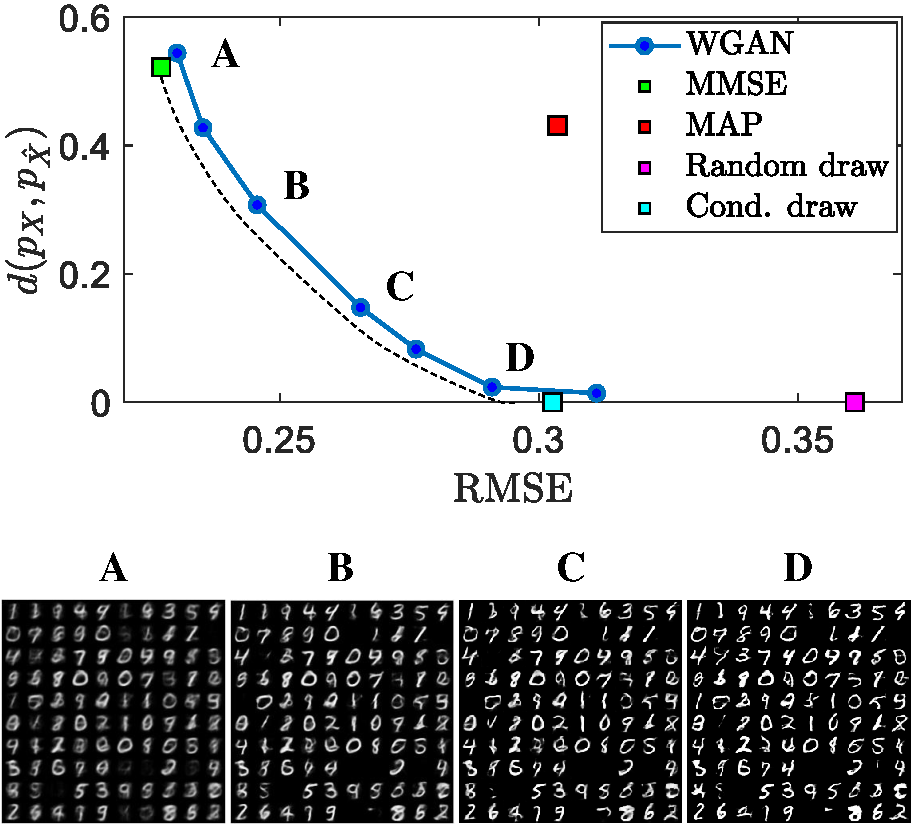
\includegraphics[width=\linewidth]{figures/WGAN.pdf}
	\end{center}
	\caption{\textbf{Image denoising utilizing a GAN.} A Wasserstein GAN was trained to denoise the images of the experiment in Fig.~\ref{fig:MMSE_MAP}. The generator loss $l_\text{gen} = l_{\text{MSE}} + \lambda \, l_{\text{adv}}$ consists of a perceptual quality (adversarial) loss and a distortion (MSE) loss, where $\lambda$ controls the trade-off between the two. For each $\lambda \in [0,0.3]$, the graph depicts the distortion (MSE) and perceptual quality (Wasserstein distance between $p_X$ and $p_{\hat{X}}$). The curve connecting the estimators is a good approximation to the theoretical perception-distortion tradeoff (illustrated by a dashed line).}
	\label{fig:WGAN}
\end{figure}

Besides the MMSE estimator, Figure \ref{fig:WGAN} also includes the MAP estimator, the random draw estimator $\hat{x}\sim p_X$ (which ignores the noisy image $y$), and the conditional draw estimator of \eqref{eq:xpost}. The perceptual quality of these estimators is evaluated, as above, by the final loss of the WGAN discriminator \cite{arjovsky2017wasserstein}, trained (without a generator) to distinguish between the estimators' outputs and images from the dataset.
Note that the denoising WGAN estimator (D) achieves the same distortion as the MAP estimator, but with far better perceptual quality. Furthermore, it achieves nearly the same perceptual quality as the random draw estimator, but with a significantly lower distortion.
